\chapter{Contoh Data dan Hasil Evaluasi}
\label{chapter:contoh-data}

\section{Hasil Evaluasi Model pada Data QRIS}

\begin{table}[htbp]
    \centering
    \begin{tabularx}{\textwidth}{|p{4.2cm}|X|X|}
        \hline
        \textbf{Data Gambar} & \textbf{Kondisi} & \textbf{Hasil Ekstraksi} \\ \hline
        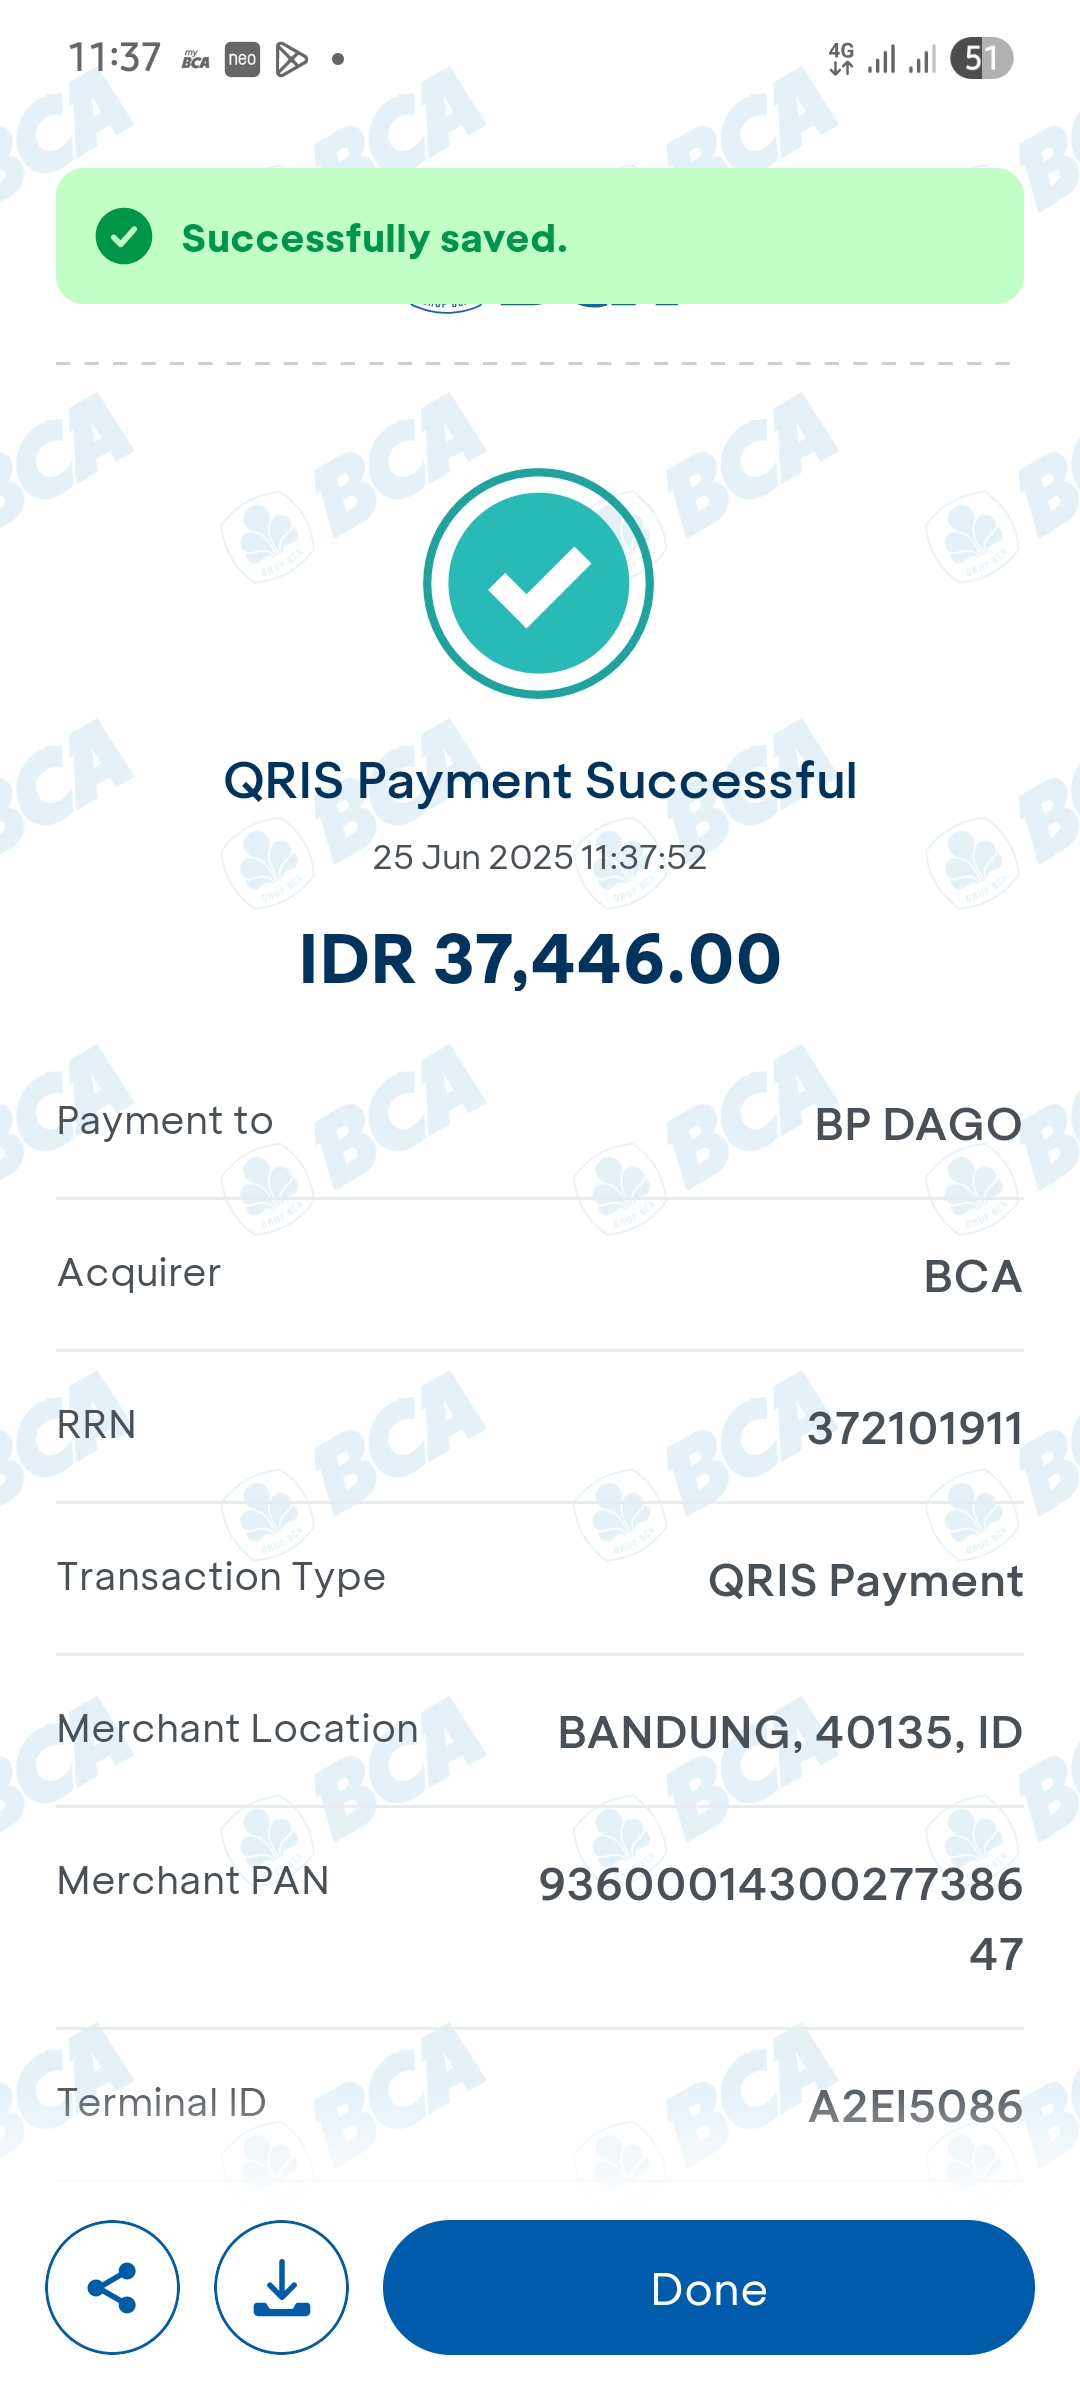
\includegraphics[width=0.25\textwidth]{images/contoh-data/qris-1.jpg} & 
         & 
         \\ \hline
        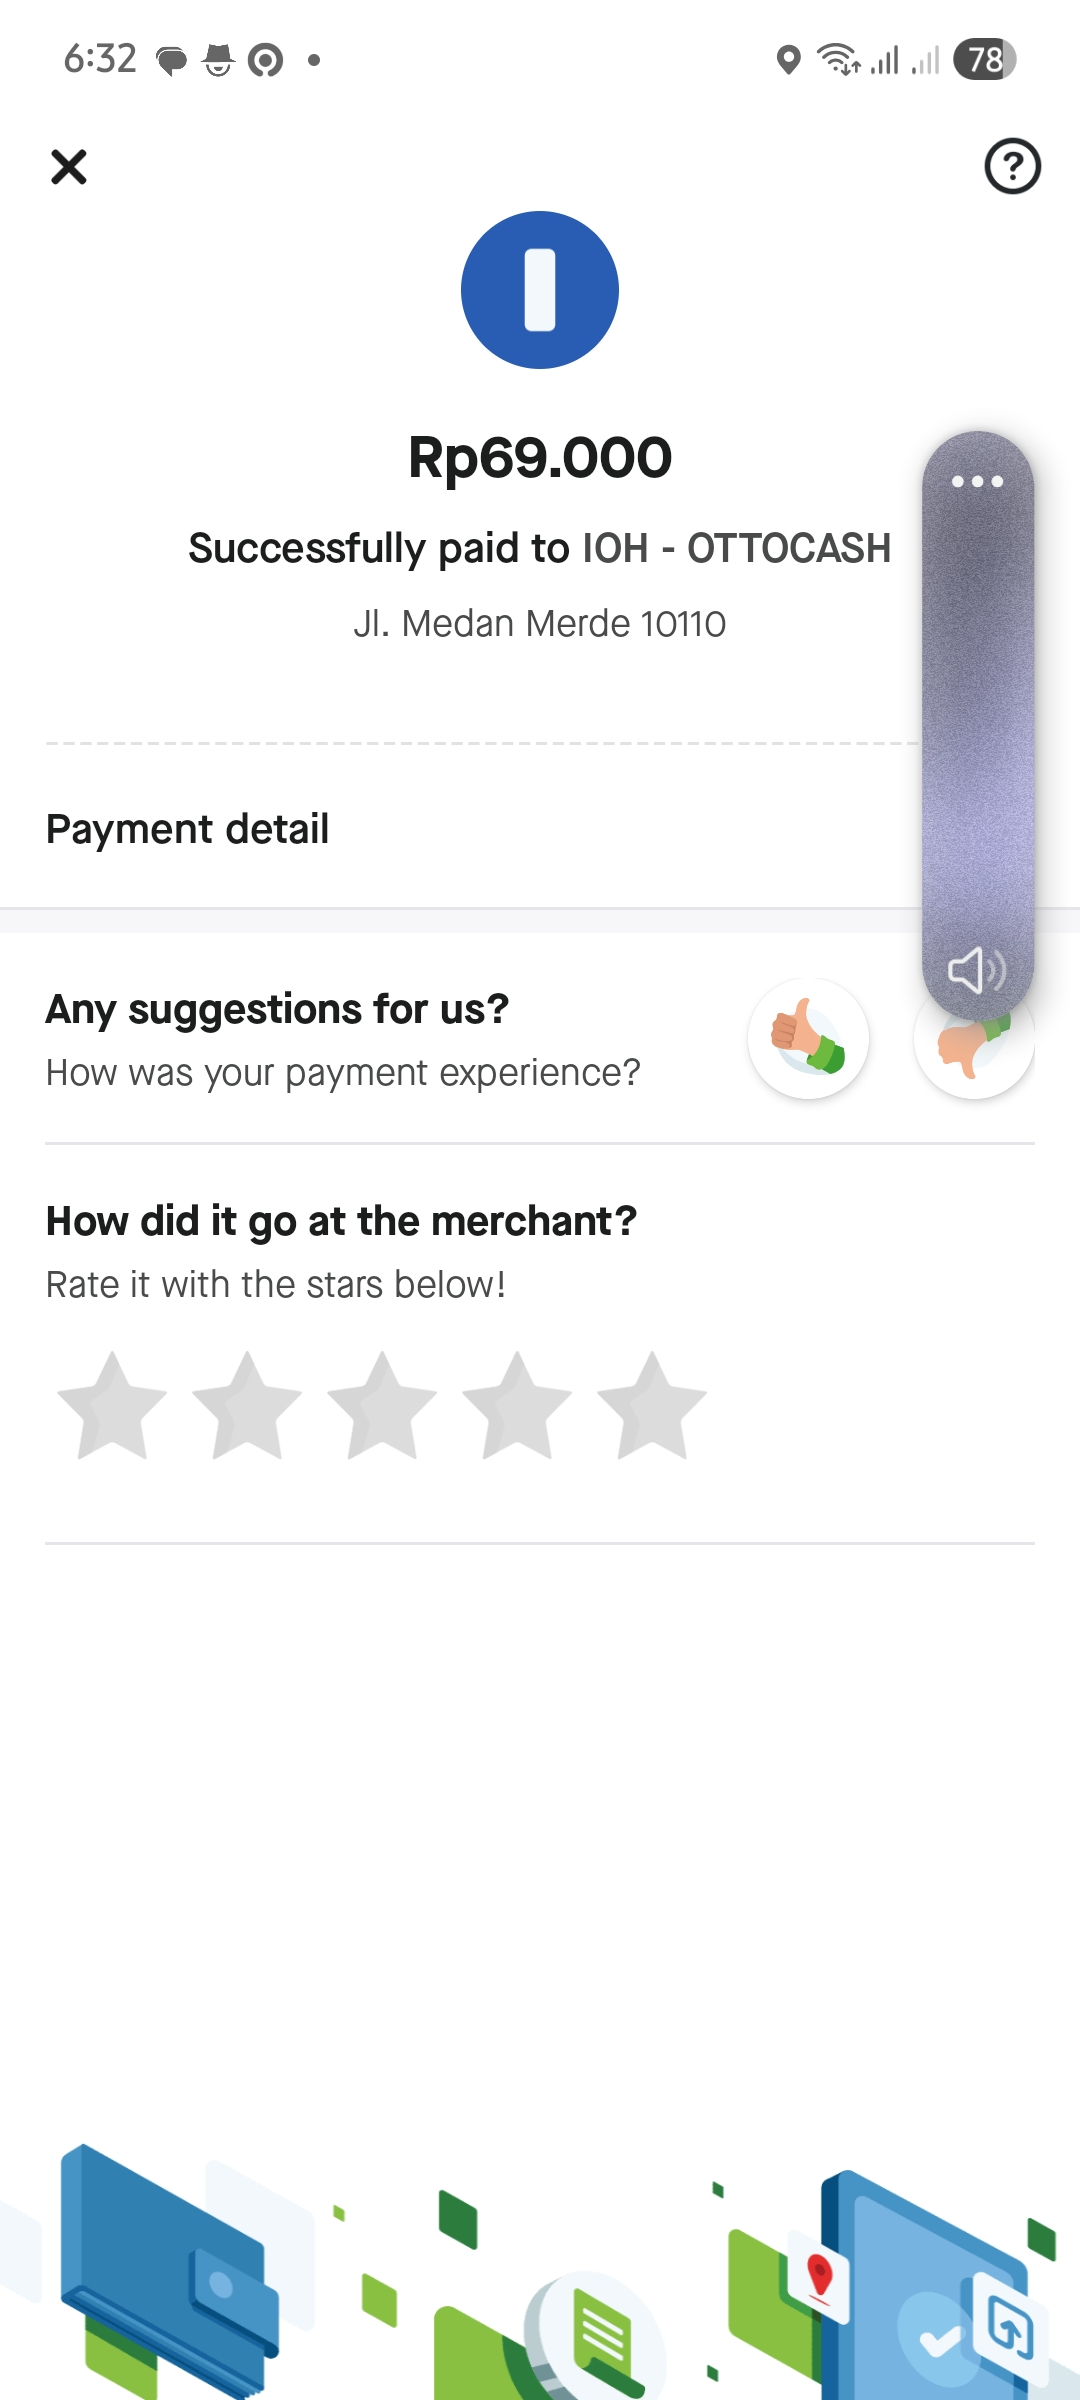
\includegraphics[width=0.25\textwidth]{images/contoh-data/qris-2.jpg} & 
         & 
         \\ \hline
    \end{tabularx}
\end{table}

\begin{table}[htbp]
    \centering
    \begin{tabularx}{\textwidth}{|p{4.2cm}|X|X|}
        \hline
        \textbf{Data Gambar} & \textbf{Kondisi} & \textbf{Hasil Ekstraksi} \\ \hline
        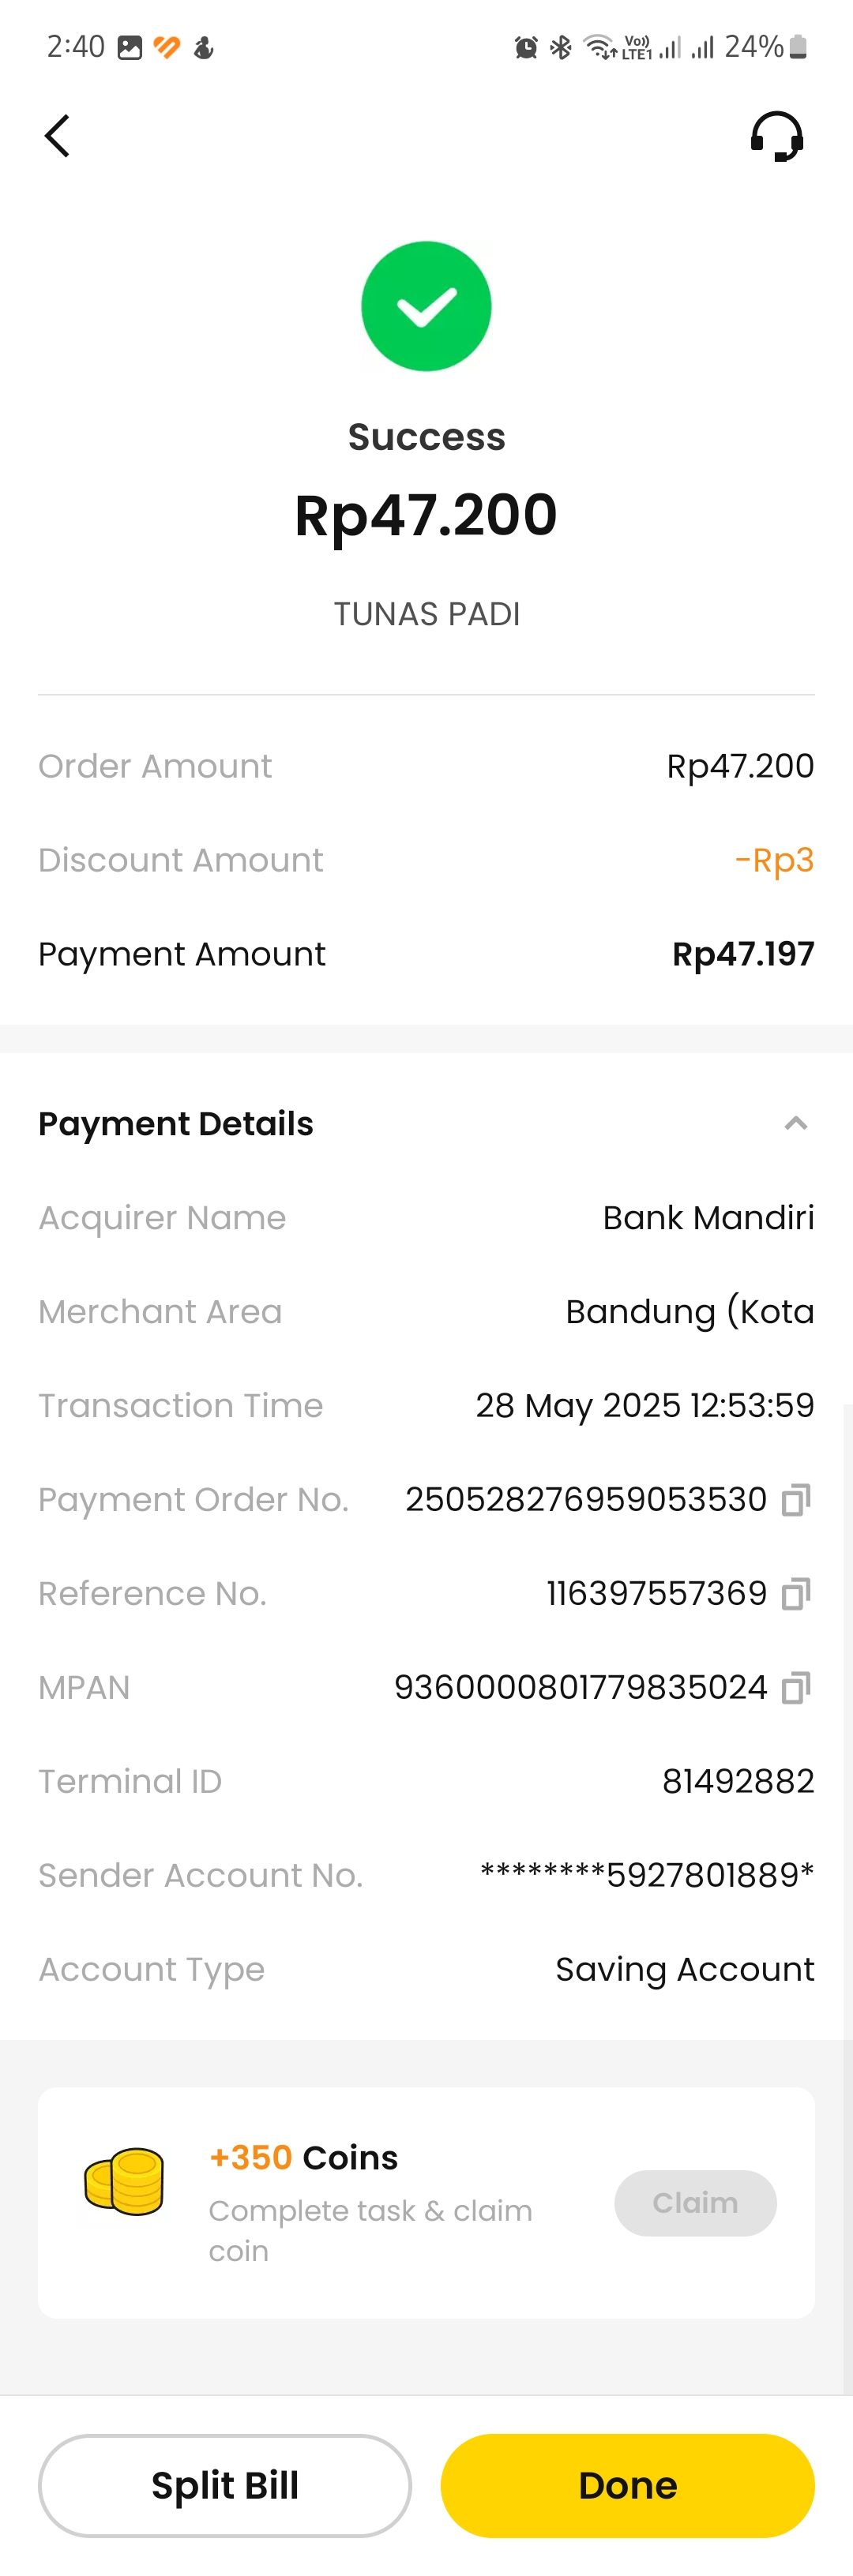
\includegraphics[width=0.25\textwidth]{images/contoh-data/qris-3.jpg} & 
         & 
         \\ \hline
        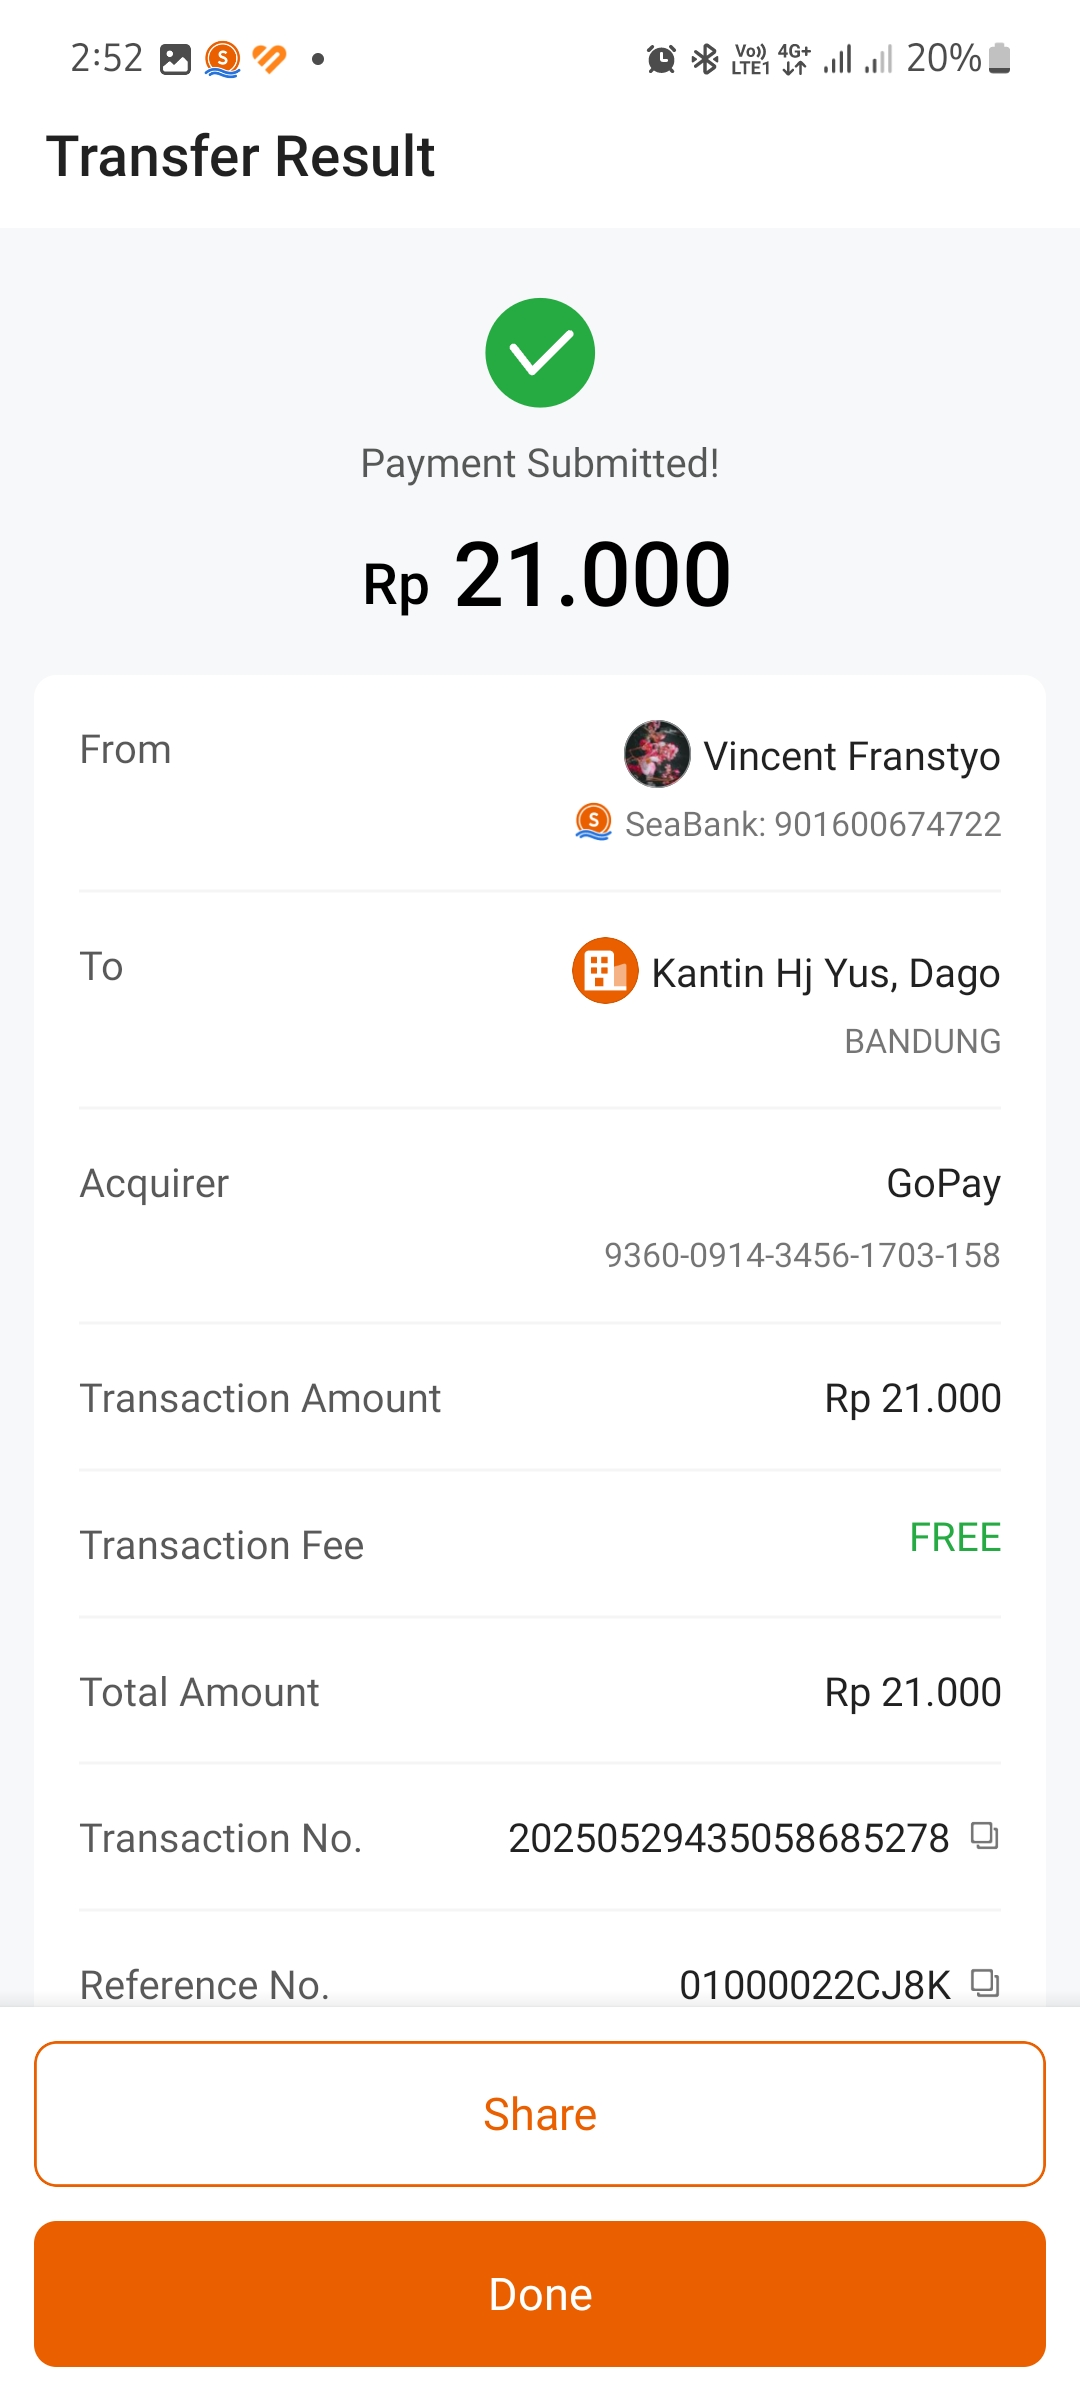
\includegraphics[width=0.25\textwidth]{images/contoh-data/qris-4.jpg} & 
         & 
         \\ \hline
    \end{tabularx}
\end{table}

\newpage

\section{Hasil Evaluasi Model pada Data Transfer}

\begin{table}[htbp]
    \centering
    \begin{tabularx}{\textwidth}{|p{4.2cm}|X|X|X|}
        \hline
        \textbf{Data Gambar} & \textbf{Kondisi} & \textbf{Hasil Ekstraksi} \\ \hline
        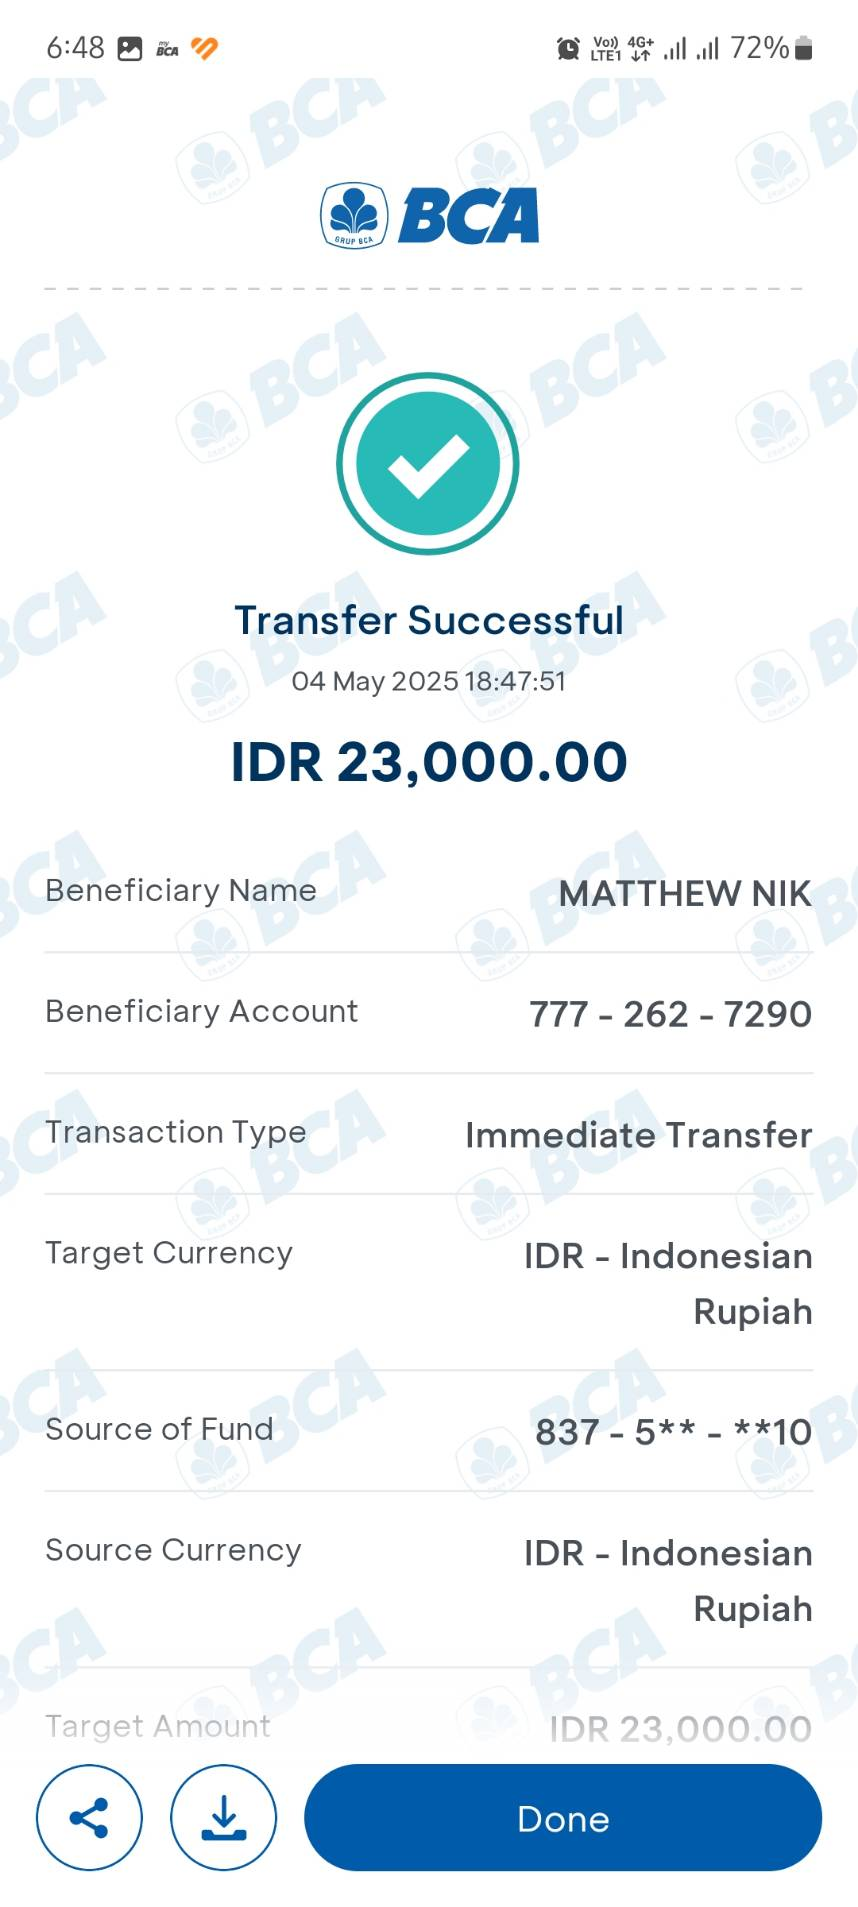
\includegraphics[width=0.3\textwidth]{images/contoh-data/tf-1.jpg} & 
         & 
         \\ \hline
        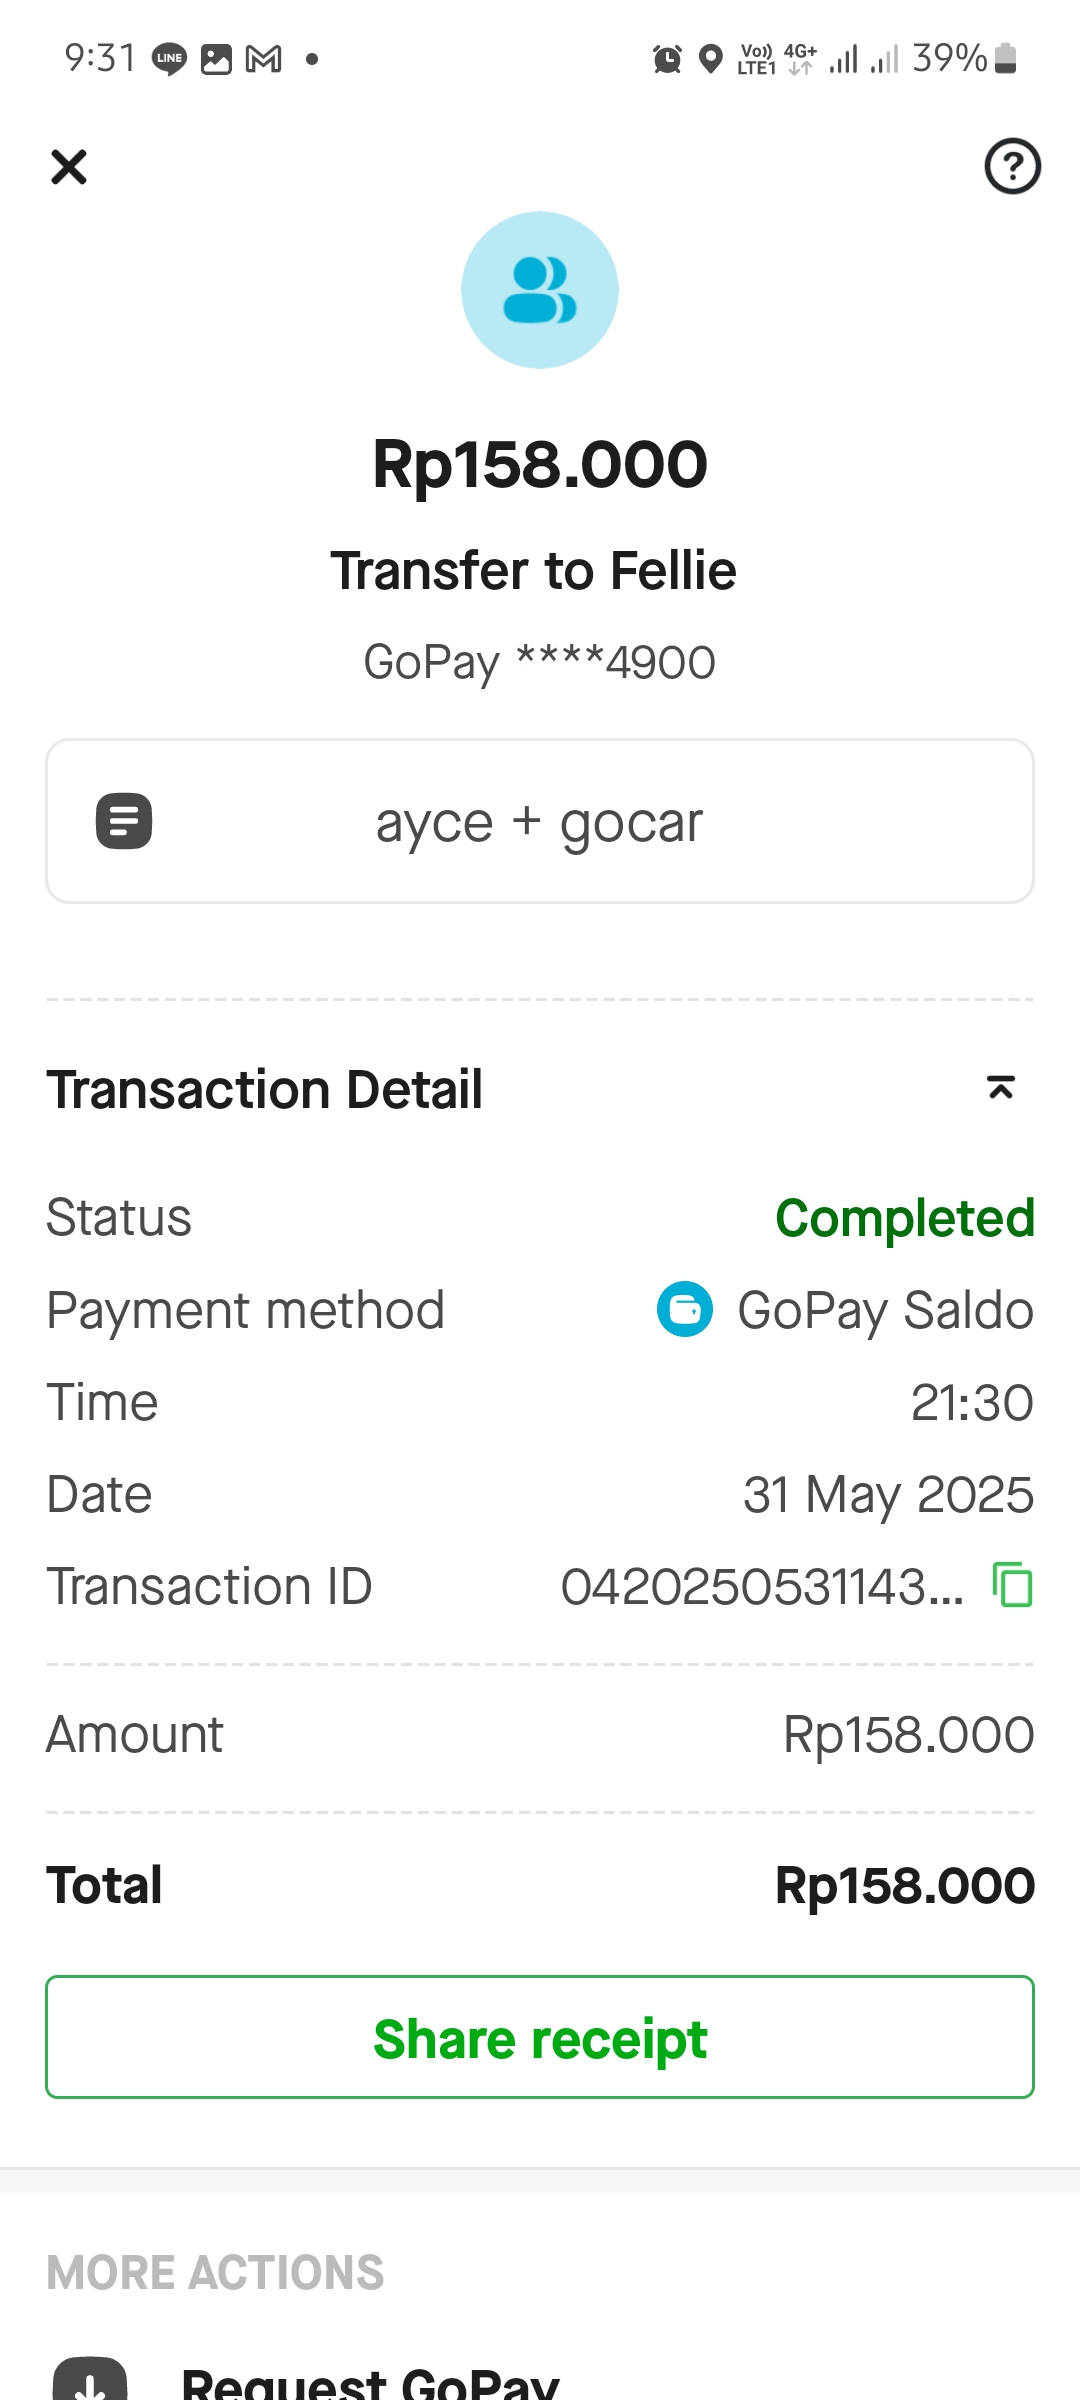
\includegraphics[width=0.3\textwidth]{images/contoh-data/tf-2.jpg} & 
         & 
         \\ \hline
    \end{tabularx}
\end{table}

\begin{table}[htbp]
    \centering
    \begin{tabularx}{\textwidth}{|p{4.2cm}|X|X|}
        \hline
        \textbf{Data Gambar} & \textbf{Kondisi} & \textbf{Hasil Ekstraksi}\\ \hline
        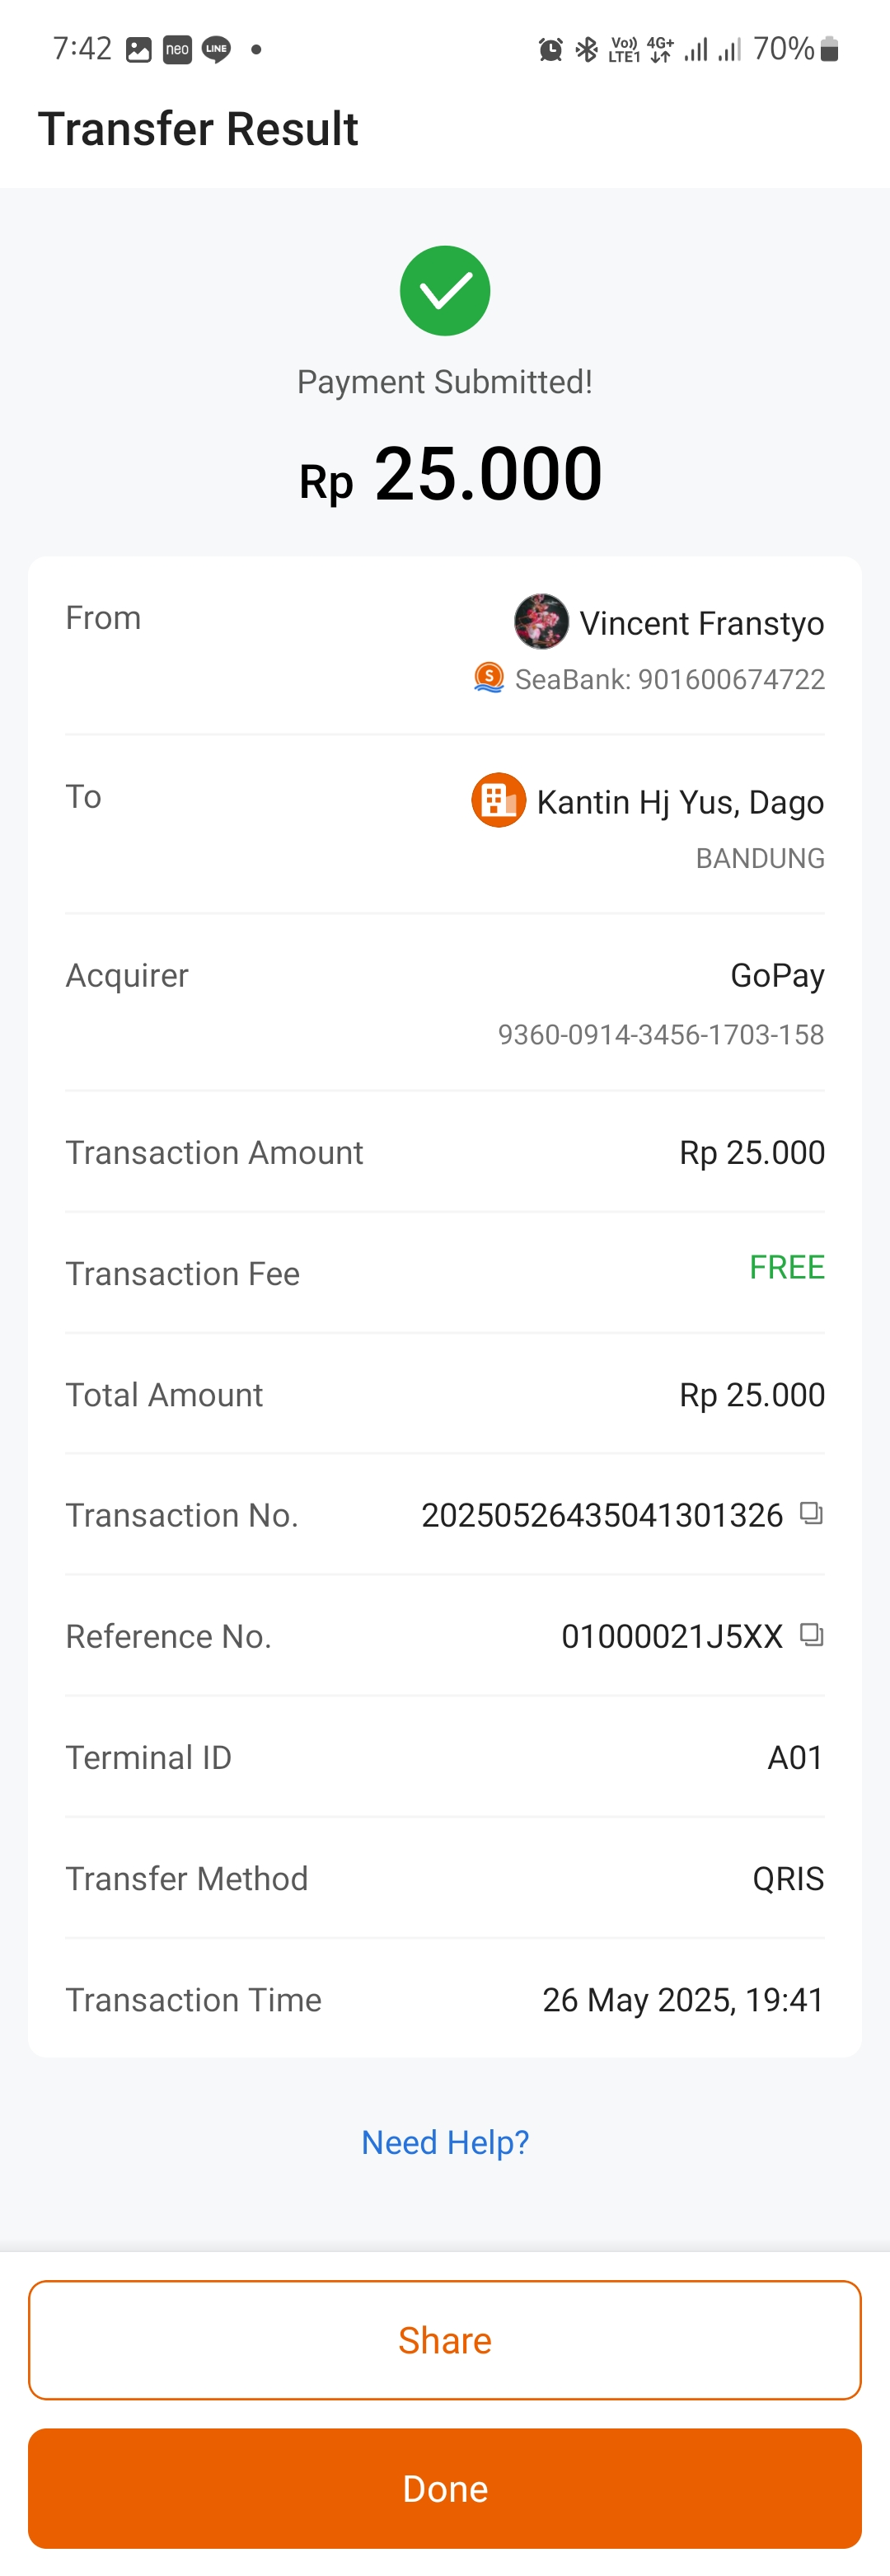
\includegraphics[width=0.3\textwidth]{images/contoh-data/tf-3.jpg} & 
         & 
         \\ \hline
        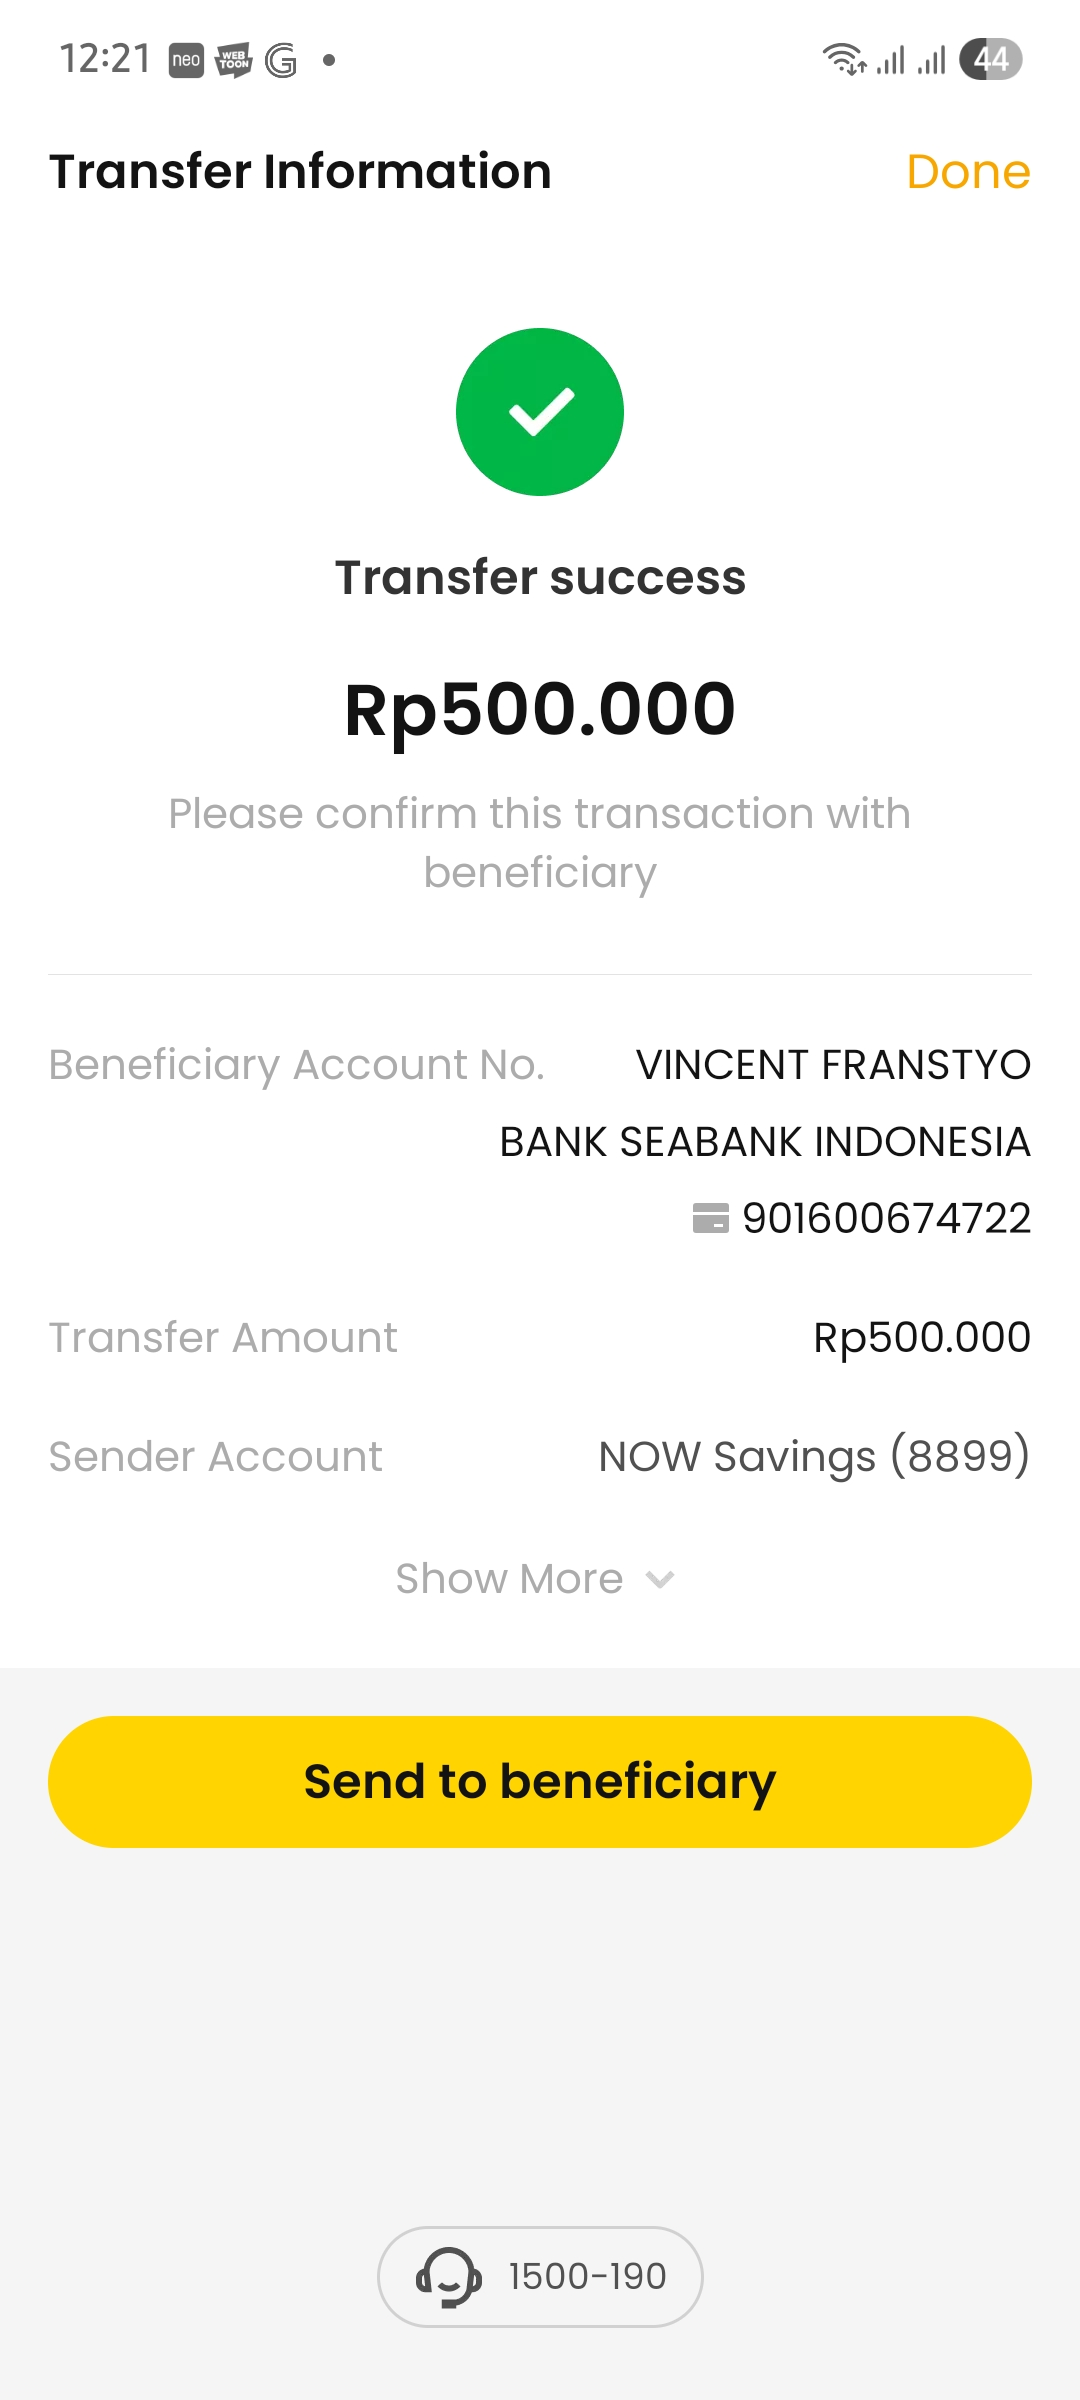
\includegraphics[width=0.3\textwidth]{images/contoh-data/tf-4.jpg} & 
         & 
         \\ \hline
    \end{tabularx}
\end{table}

\newpage

\section{Hasil Evaluasi Model pada Data Struk}

\begin{table}[htbp]
    \centering
    \begin{tabularx}{\textwidth}{|p{4.2cm}|X|X|}
        \hline
        \textbf{Data Gambar} & \textbf{Kondisi} & \textbf{Hasil Ekstraksi}\\ \hline
        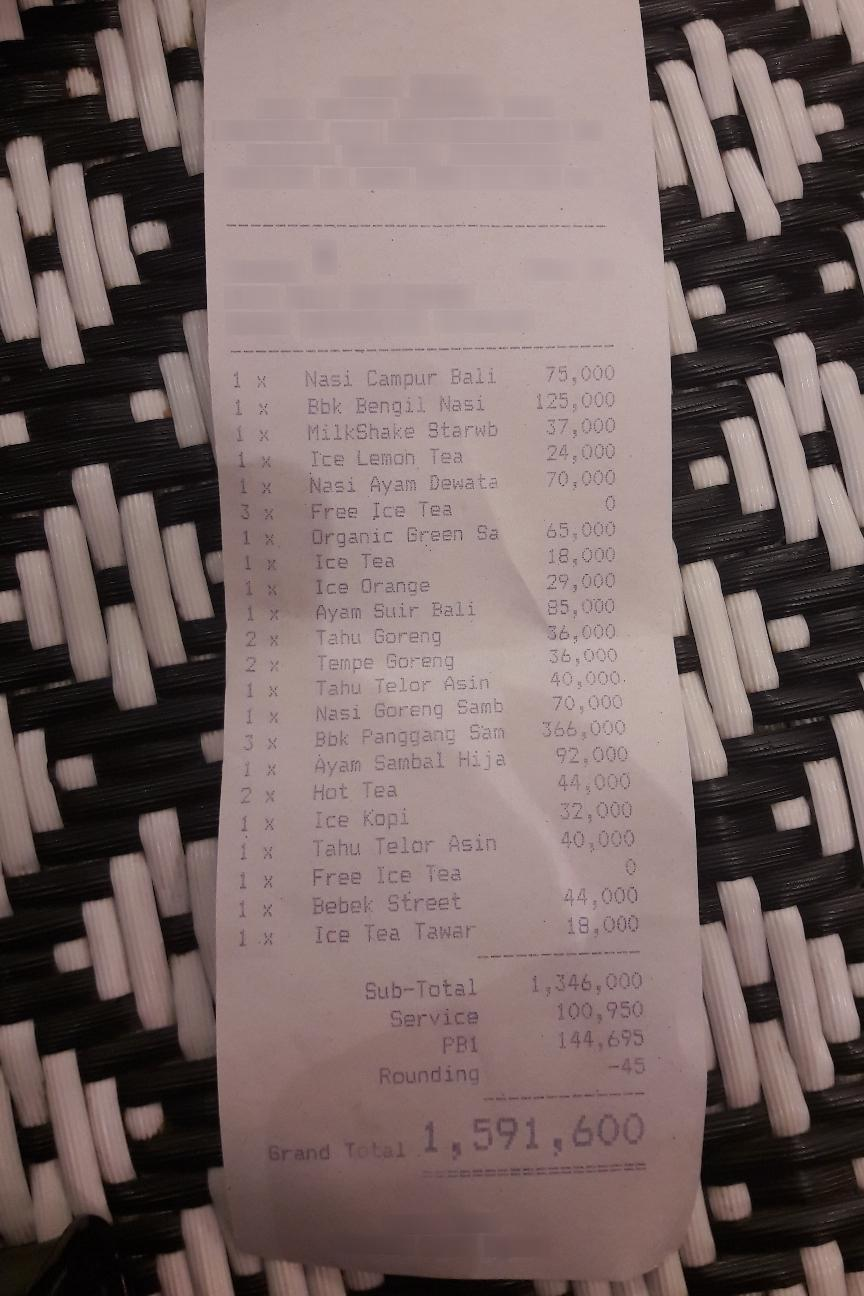
\includegraphics[width=0.3\textwidth]{images/contoh-data/struk-1.jpg} & 
         & 
         \\ \hline
        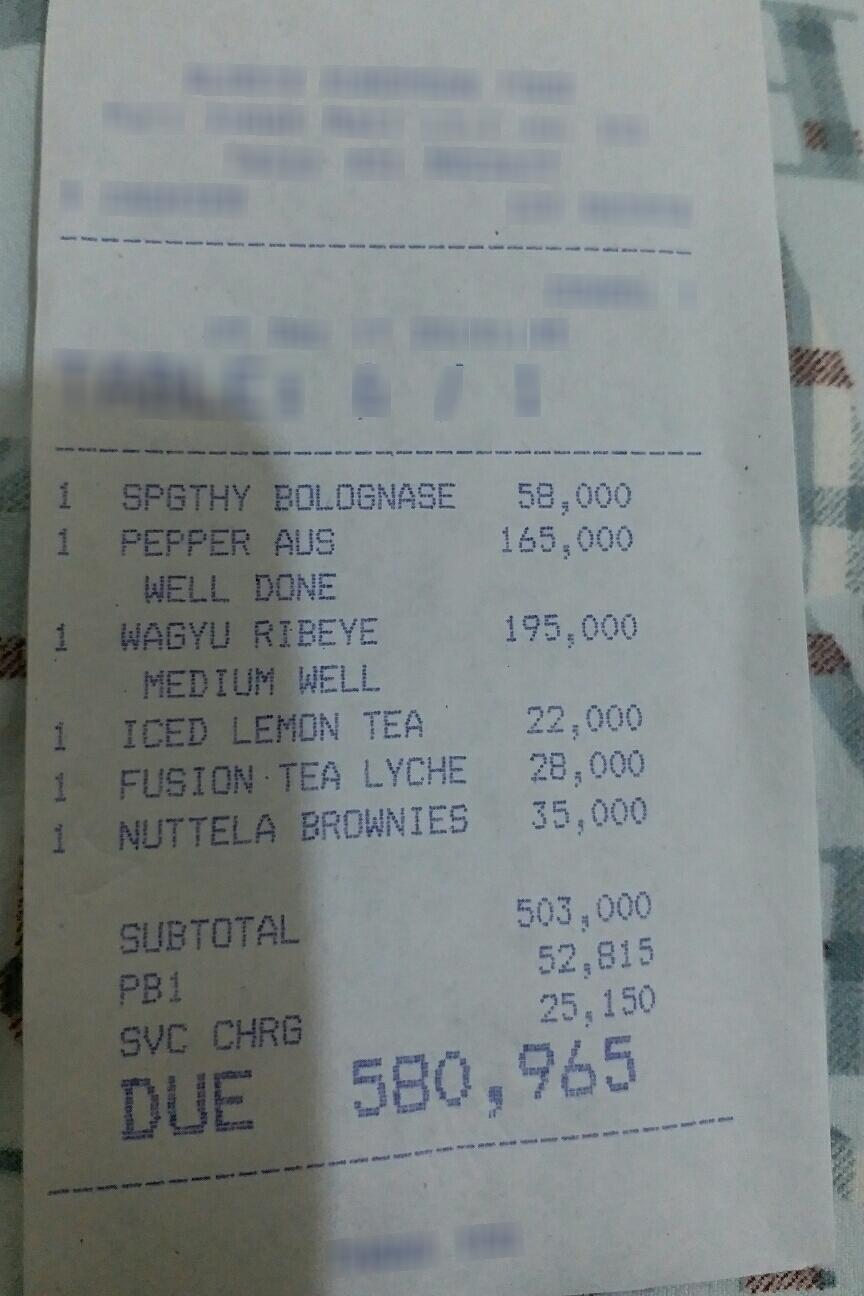
\includegraphics[width=0.3\textwidth]{images/contoh-data/struk-2.jpg} & 
         & 
         \\ \hline
        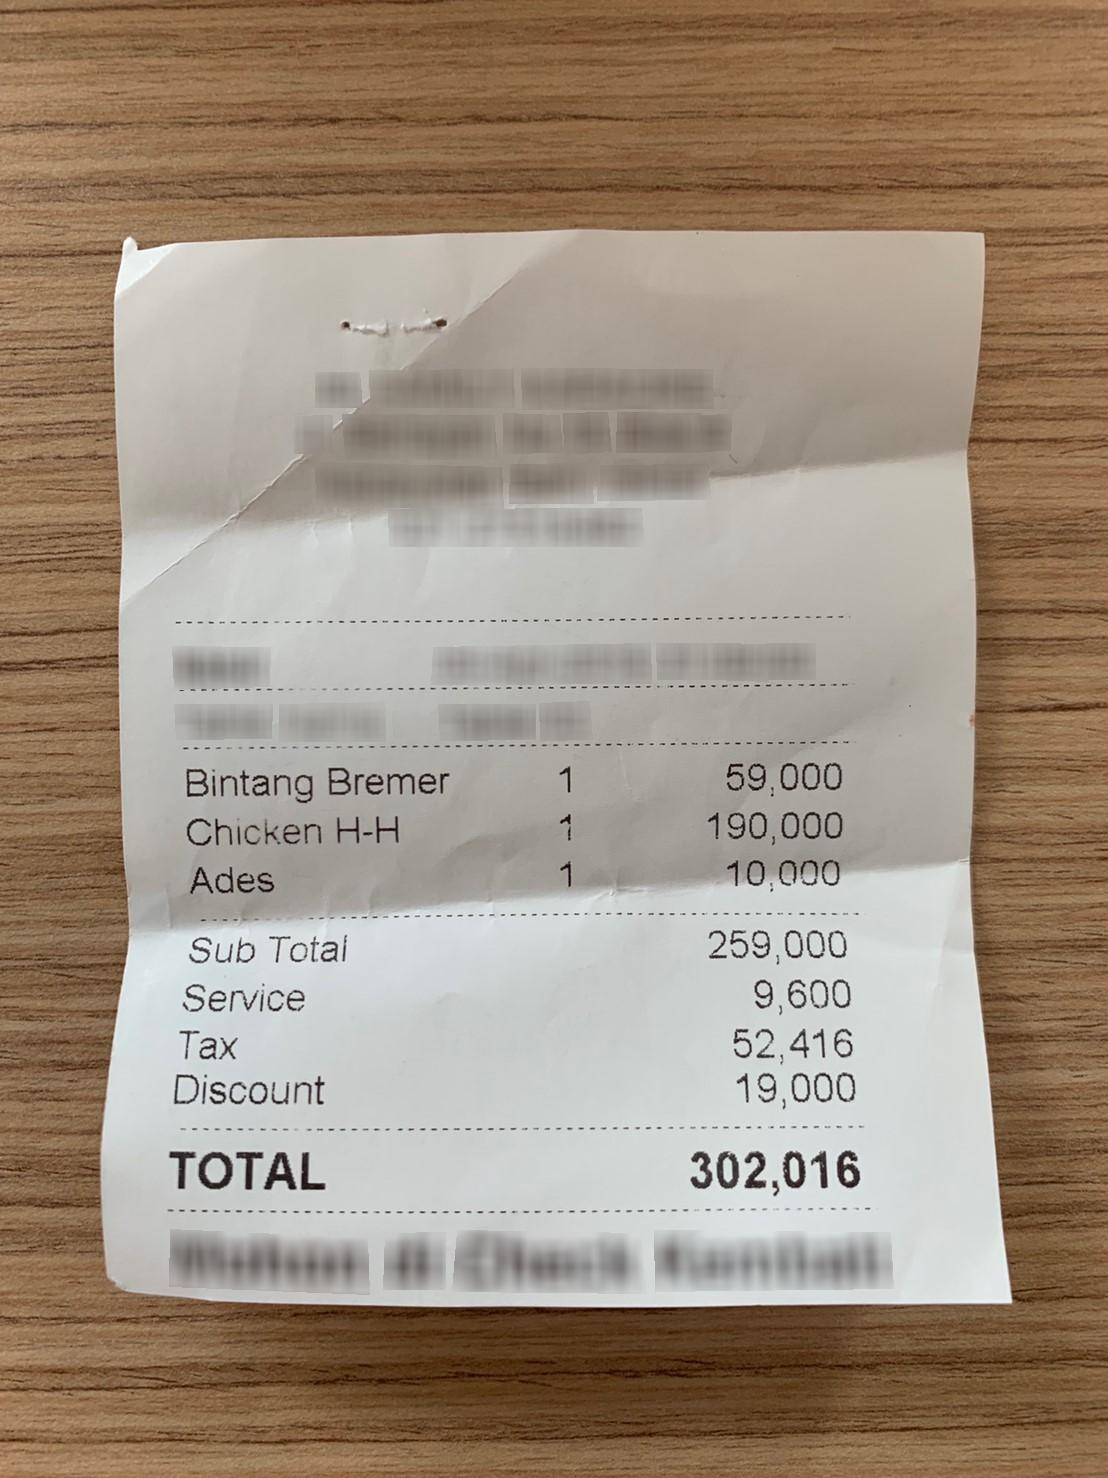
\includegraphics[width=0.3\textwidth]{images/contoh-data/struk-3.jpg} & 
         & 
         \\ \hline
    \end{tabularx}
\end{table}

\begin{table}[htbp]
    \centering
    \begin{tabularx}{\textwidth}{|p{4.2cm}|X|X|}
        \hline
        \textbf{Data Gambar} & \textbf{Kondisi} & \textbf{Hasil Ekstraksi}\\ \hline
        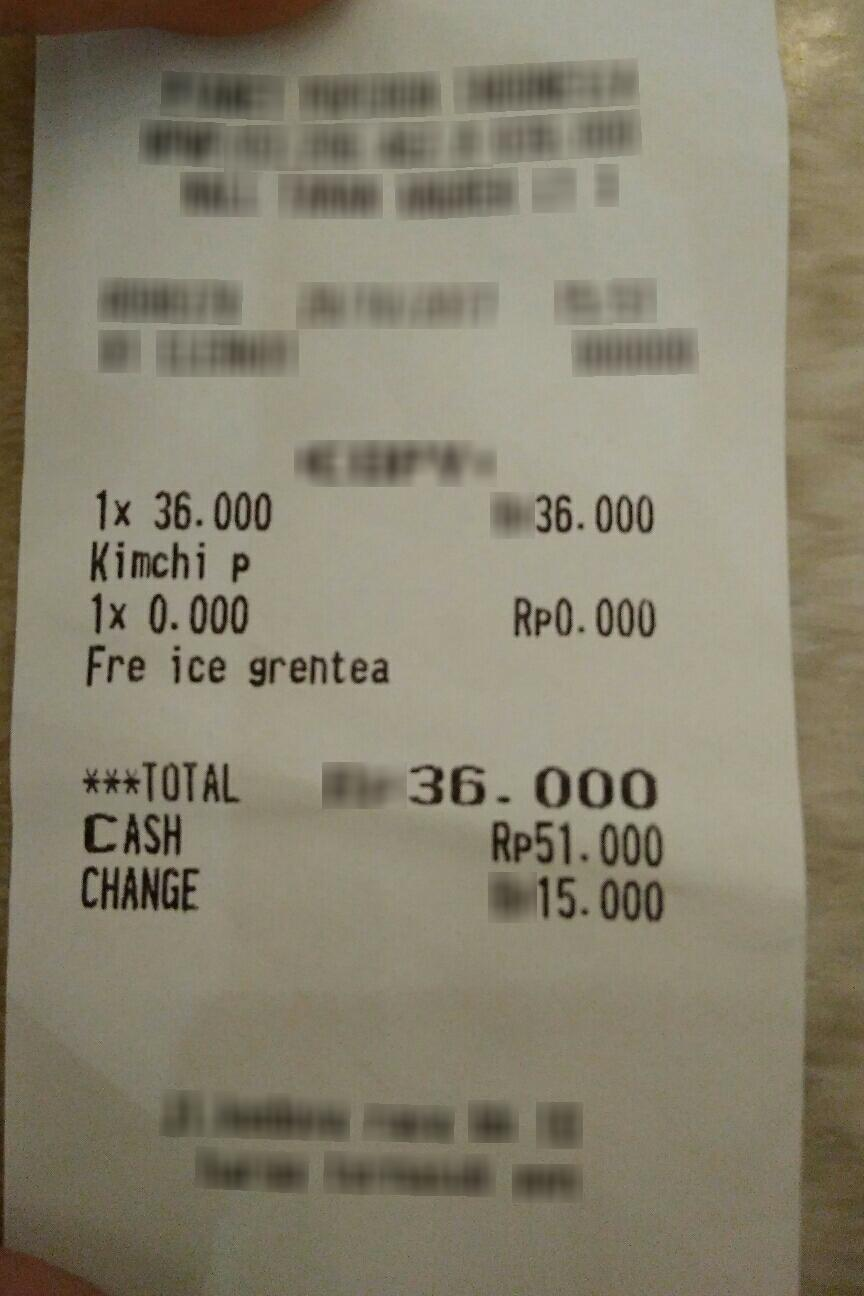
\includegraphics[width=0.3\textwidth]{images/contoh-data/struk-4.jpg} & 
         & 
         \\ \hline
    \end{tabularx}
\end{table}